\documentclass[a4paper, 11pt]{article}

\usepackage[left=1.5cm, right=1.5cm, top=2cm, bottom=2cm]{geometry}

\usepackage[utf8]{inputenc} 
\usepackage[T1]{fontenc}      
\usepackage[french,english]{babel}  
\usepackage{lmodern}

\usepackage{amsmath, mathtools}
\usepackage{amssymb}
\usepackage{amsthm}
\usepackage{empheq}

\usepackage{graphicx}
\usepackage{subfig}

\usepackage{listings}
\usepackage{color} %red, green, blue, yellow, cyan, magenta, black, white
\definecolor{mygreen}{RGB}{28,172,0} % color values Red, Green, Blue
\definecolor{mylilas}{RGB}{170,55,241}

\usepackage{mathtools}
\DeclarePairedDelimiter\ceil{\lceil}{\rceil}

\lstset{language=Matlab,%
    %basicstyle=\color{red},
    breaklines=true,%
    morekeywords={matlab2tikz},
    keywordstyle=\color{blue},%
    morekeywords=[2]{1}, keywordstyle=[2]{\color{black}},
    identifierstyle=\color{black},%
    stringstyle=\color{mylilas},
    commentstyle=\color{mygreen},%
    showstringspaces=false,%without this there will be a symbol in the places where there is a space
    numbers=left,%
    numberstyle={\tiny \color{black}},% size of the numbers
    numbersep=9pt, % this defines how far the numbers are from the text
    emph=[1]{for,end,break},emphstyle=[1]\color{red}, %some words to emphasise
    %emph=[2]{word1,word2}, emphstyle=[2]{style},    
}

\begin{document}
\title{Rendu TP2 Image sous-pixellique}
\author{Yoann Pradat}
\maketitle

\paragraph{Exercice 4}

%%%%%%%%%%%%
% Question 1
%%%%%%%%%%%%

1)
\begin{lstlisting}[frame=single]
u = double(imread("room.pgm"))/255;
imshow(u);

lambda=3;
v = u(1:lambda:end, 1:lambda:end);
w = kron(v, ones(lambda));
[ny, nx] = size(u);
imshow([u, w(1:ny, 1:nx)]);
\end{lstlisting}

On charge l'image 512x512 room.pgm et on l'affiche. A coté de cette image on va afficher une autre image de même taille.
Cette seconde image est créée à partir de la première en échantillonnant avec un pas de $\lambda$. Pour $\lambda$ = 3 par
exemple, le premier carré de pixels [1,3]x[1,3] est réduit au pixel [1,1]. \\

Plus généralement, le carré de pixels [(k-1)*$\lambda$+ 1, k*$\lambda$]x[(l-1)*$\lambda$+ 1, l*$\lambda$] est réduit au
pixel [(k-1)*$\lambda$+ 1, (l-1)*$\lambda$+ 1] pour k, l = 1, $\dots$, $\ceil{\frac{512}{\lambda}}$. \\

L'image échantillonnée est enregistrée dans la matrice v, qui est de taille
$\ceil{\frac{512}{\lambda}}$x$\ceil{\frac{512}{\lambda}}$. 
Pour comparer à l'image de base, on fait un zoom de la manière suivante: on recrée le carré de pixels [(k-1)*$\lambda$ +
1, k*$\lambda$]x[(l-1)*$\lambda$ 1, l*$\lambda$] en mettant tous ces pixels à la valeur échantillonnée [k-1, l-1]: c'est
la matrice w.

\begin{figure}[!h]
\centering
\includegraphics[width=10cm]{room.png}
\caption{(g.) Image de base. (d.) son échantillonnée zoomée avec pas $\lambda$=3}
\end{figure}

%%%%%%%%%%%%
% Question 2
%%%%%%%%%%%%

2) Le phénomène observé est appelé \textbf{aliasing}. Il y en a plusieurs manifestations sur cette image:
\begin{itemize}
  \item en bas à gauche, le motif strié voit ses stries orientées dans une autre direction. Si on modélise les stries
    par une onde pure, le vecteur directeur \textbf{k} de cette onde a été aliasé en \textbf{k'}.
  \item en haut à gauche, le fil n'est plus continu, on a perte de connexité. 
  \item à droite par exemple, les bords des objets comme le rideau (zone de forte contraste) sont ``en escalier'' au
    lieu d'être rectilignes.
\end{itemize}

%%%%%%%%%%%%
% Question 3
%%%%%%%%%%%%
\pagebreak
3)
\begin{lstlisting}[frame=single]
f = zeros(512);
f(190, 50) = 2;
onde = real(ifft2(f));
imshow(onde, []);

onde_ft = abs(fft2(onde));
imshow(fftshift(onde_ft), [0,max(max(onde_ft))], 'xdata', 1:512, 'ydata', 1:512);
axis on;
\end{lstlisting}


On visualise l'onde créée en utilisant imshow et on visualise également sa transformée de Fourier recentrée de telle
sorte que la ``fréquence 0'' soit au centre de l'image. 

\begin{figure}[!h]
\centering
\subfloat[L'onde pure]{{\includegraphics[width=8cm]{onde.png}}}%
\qquad
\subfloat[Transformée de Fourier discrète recentrée]{{\includegraphics[width=8cm]{onde_ft.png}}}%
\end{figure}

En explicitant les transformation de Fourier discrètes on a:
\begin{align}
\forall p, q \in 1,\dots,512 \qquad \text{onde}[p,q] &= \Re{\Big(\frac{2}{512^2} e^{\frac{2i\pi189(p-1)}{512}}
  e^{\frac{2i\pi49(q-1)}{512}}\Big)} \\
\text{onde}_{\text{ft}}[p,q] &= \left| \sum_{j=0}^{511} \sum_{k=0}^{511} e^{-\frac{2i\pi(p-1)j}{512}}
e^{\frac{-2i\pi(q-1)k}{512}} \text{onde}[j,k] \right|
\end{align}

On montre aisément qu'il y a exactement 2 points sur le domaine [1, 512]x[1, 512] pour lesquels $\text{onde}_{\text{ft}}$
n'est pas nulle, ce sont les points de coordonnées matricielles [p,q] = [190, 50] et [p,q] = [512-190, 512-50] soit en 
coordonnées d'image non recentrées [x,y]=[50,190] et [x,y] = [462, 322]. Après recentrage par la fonction \textit{fftshift}
les deux points non nuls sur l'image bidimensionnelle b) de la transformée de Fourier de l'onde ont pour coordonnées
[x,y] = [206, 66] et [x,y]=[306, 446]. En sachant que la fréquence 0 du spectre est au centre de l'image, on
obtient que les deux seuls points du spectre où la transformée de Fourier n'est pas nulle sont [50, -190] et [-50,
190].\\ 

\pagebreak

Echantillonnons l'image de l'onde pure avec un pas de 2. De même qu'à la question 1 on zoome l'image échantillonnée par
un procédé très simple et on affiche les deux images côte à côte:

\begin{figure}[!h]
\centering
\includegraphics[width=10cm]{onde_onde_ech.png}
\caption{(g.) Image de base. (d.) son échantillonnée zoomée avec pas $\lambda$=2}
\end{figure}

On observe l'aliasing par un changement dans le vecteur directeur de l'onde pure reconstruite par échantillonnage. \\

\begin{lstlisting}[frame=single]
% Sous échantillonnage facteur 2 onde
lambda=2;
onde_ech = onde(1:lambda:end, 1:lambda:end);
onde_ech_zoom = kron(onde_ech, ones(lambda));
[ny, nx] = size(onde);

% Onde échantillonée et transfo fourier
onde_ech_ft = abs(fft2(onde_ech));
imshow(fftshift(onde_ech_ft), [0,max(max(onde_ech_ft))], 'xdata', 1:256, 'ydata', 1:256);
axis on;
\end{lstlisting}

Intéressons-nous désormais à la transformée de Fourier de l'échantillonnée. L'onde échantillonnée est telle que:

\begin{align}
\forall p, q \in 1,\dots,256 \qquad \text{onde\_ech}[p,q] &= \text{onde}[2p-1, 2q-1] \\
\text{onde\_ech}_{\text{ft}}[p,q] &= \left| \sum_{j=0}^{255} \sum_{k=0}^{255} e^{-\frac{2i\pi(p-1)j}{256}}
e^{\frac{-2i\pi(q-1)k}{256}} \Re{\Big(\frac{2}{512^2} e^{\frac{2i\pi189(2j)}{512}} e^{\frac{2i\pi49(2k)}{512}}\Big)}  \right|
\end{align}

On montre encore une fois qu'il y a exactement 2 points sur le domaine [1, 256]x[1, 256] pour lesquels
$\text{onde\_ech}_{\text{ft}}$ n'est pas nulle, ce sont les points de coordonnées matricielles [p,q] = [190, 50] et
[p,q] = [68, 208] soit en coordonnées d'image non recentrées [x,y]=[50,190] et [x,y] = [206, 66]. 

\pagebreak

\begin{figure}[!h]
\centering
\subfloat[Transformée de Fourier discrète]{{\includegraphics[width=8cm]{onde_ech_ft_noshift.png}}}%
\qquad
\subfloat[Transformée de Fourier discrète recentrée]{{\includegraphics[width=8cm]{onde_ech_ft.png}}}%
\end{figure}

Après recentrage par la fonction \textit{fftshift} les deux points non nuls sur l'image bidimensionnelle de la
transformée de Fourier de l'onde échantillonnée ont pour coordonnées [x,y] = [178, 62] (vient de l'opération 
[50+128, 190-128] effectuée par \textit{fftshift}) et [x,y]=[78, 194]. En sachant que la fréquence 0 du spectre est au
centre de l'image, on obtient que les deux seuls points du spectre où la transformée de Fourier n'est pas nulle sont 
[50, 66] et [-50, -66].

\paragraph{Exercice 5}

1)
\begin{lstlisting}[frame=single]
f = zeros(512);
f(190, 50) = 2;
onde = real(ifft2(f));
onde_car = onde.^2
% Onde et son carre
imshow(onde, []);
imshow(onde_car, []);
\end{lstlisting}

\begin{figure}[!h]
\centering
\subfloat[Image onde pure]{{\includegraphics[width=6cm]{ex_5_onde.png}}}%
\qquad
\subfloat[Image avec chaque pixel élevé au carré]{{\includegraphics[width=6cm]{ex_5_onde_car.png}}}%
\end{figure}

On sait que $\text{onde}[p,q] = \frac{2}{512^2}\cos(\frac{2\pi}{512}(189, 49)(p-1,q-1)^T)$ donc : 
\begin{align}
\text{onde}[p,q]^2 &= \frac{4}{512^4}\cos^2(\frac{2\pi}{512}(189, 49)(p-1,q-1)^T)\\
&=\frac{4}{512^4} \times \frac{1}{2}\big[\cos(\frac{2\pi}{512}2\times(189, 49)(p-1,q-1)^T) + 1\big]
\end{align}

Entre les deux images, la direction de l'onde pure est totalement modifiée. Ceci s'explique par le calcul ci-dessus: on observe la somme d'une constante et d'une onde pure différente. Cette dernière a un vecteur \textbf{k} 2 fois plus grand et donc une fréquence 2 fois plus élevée.

\begin{lstlisting}[frame=single]
imshow(fftzoom(onde,2), []);
\end{lstlisting}

\begin{figure}[!h]
\centering
\includegraphics[width=6cm]{ex_5_fftzoom.png}
\caption{Image 2 fois plus résolue par zero-padding}
\end{figure}

Cette fois-ci l'onde sur l'image 2 fois plus résolue a bien conservé l'orientation de l'onde pure qu'elle représentait
avant zero-padding. Pour comprendre pourquoi, essayons de comprendre l'effet de fftzoom sur notre onde pure.

\begin{figure}[!h]
\centering
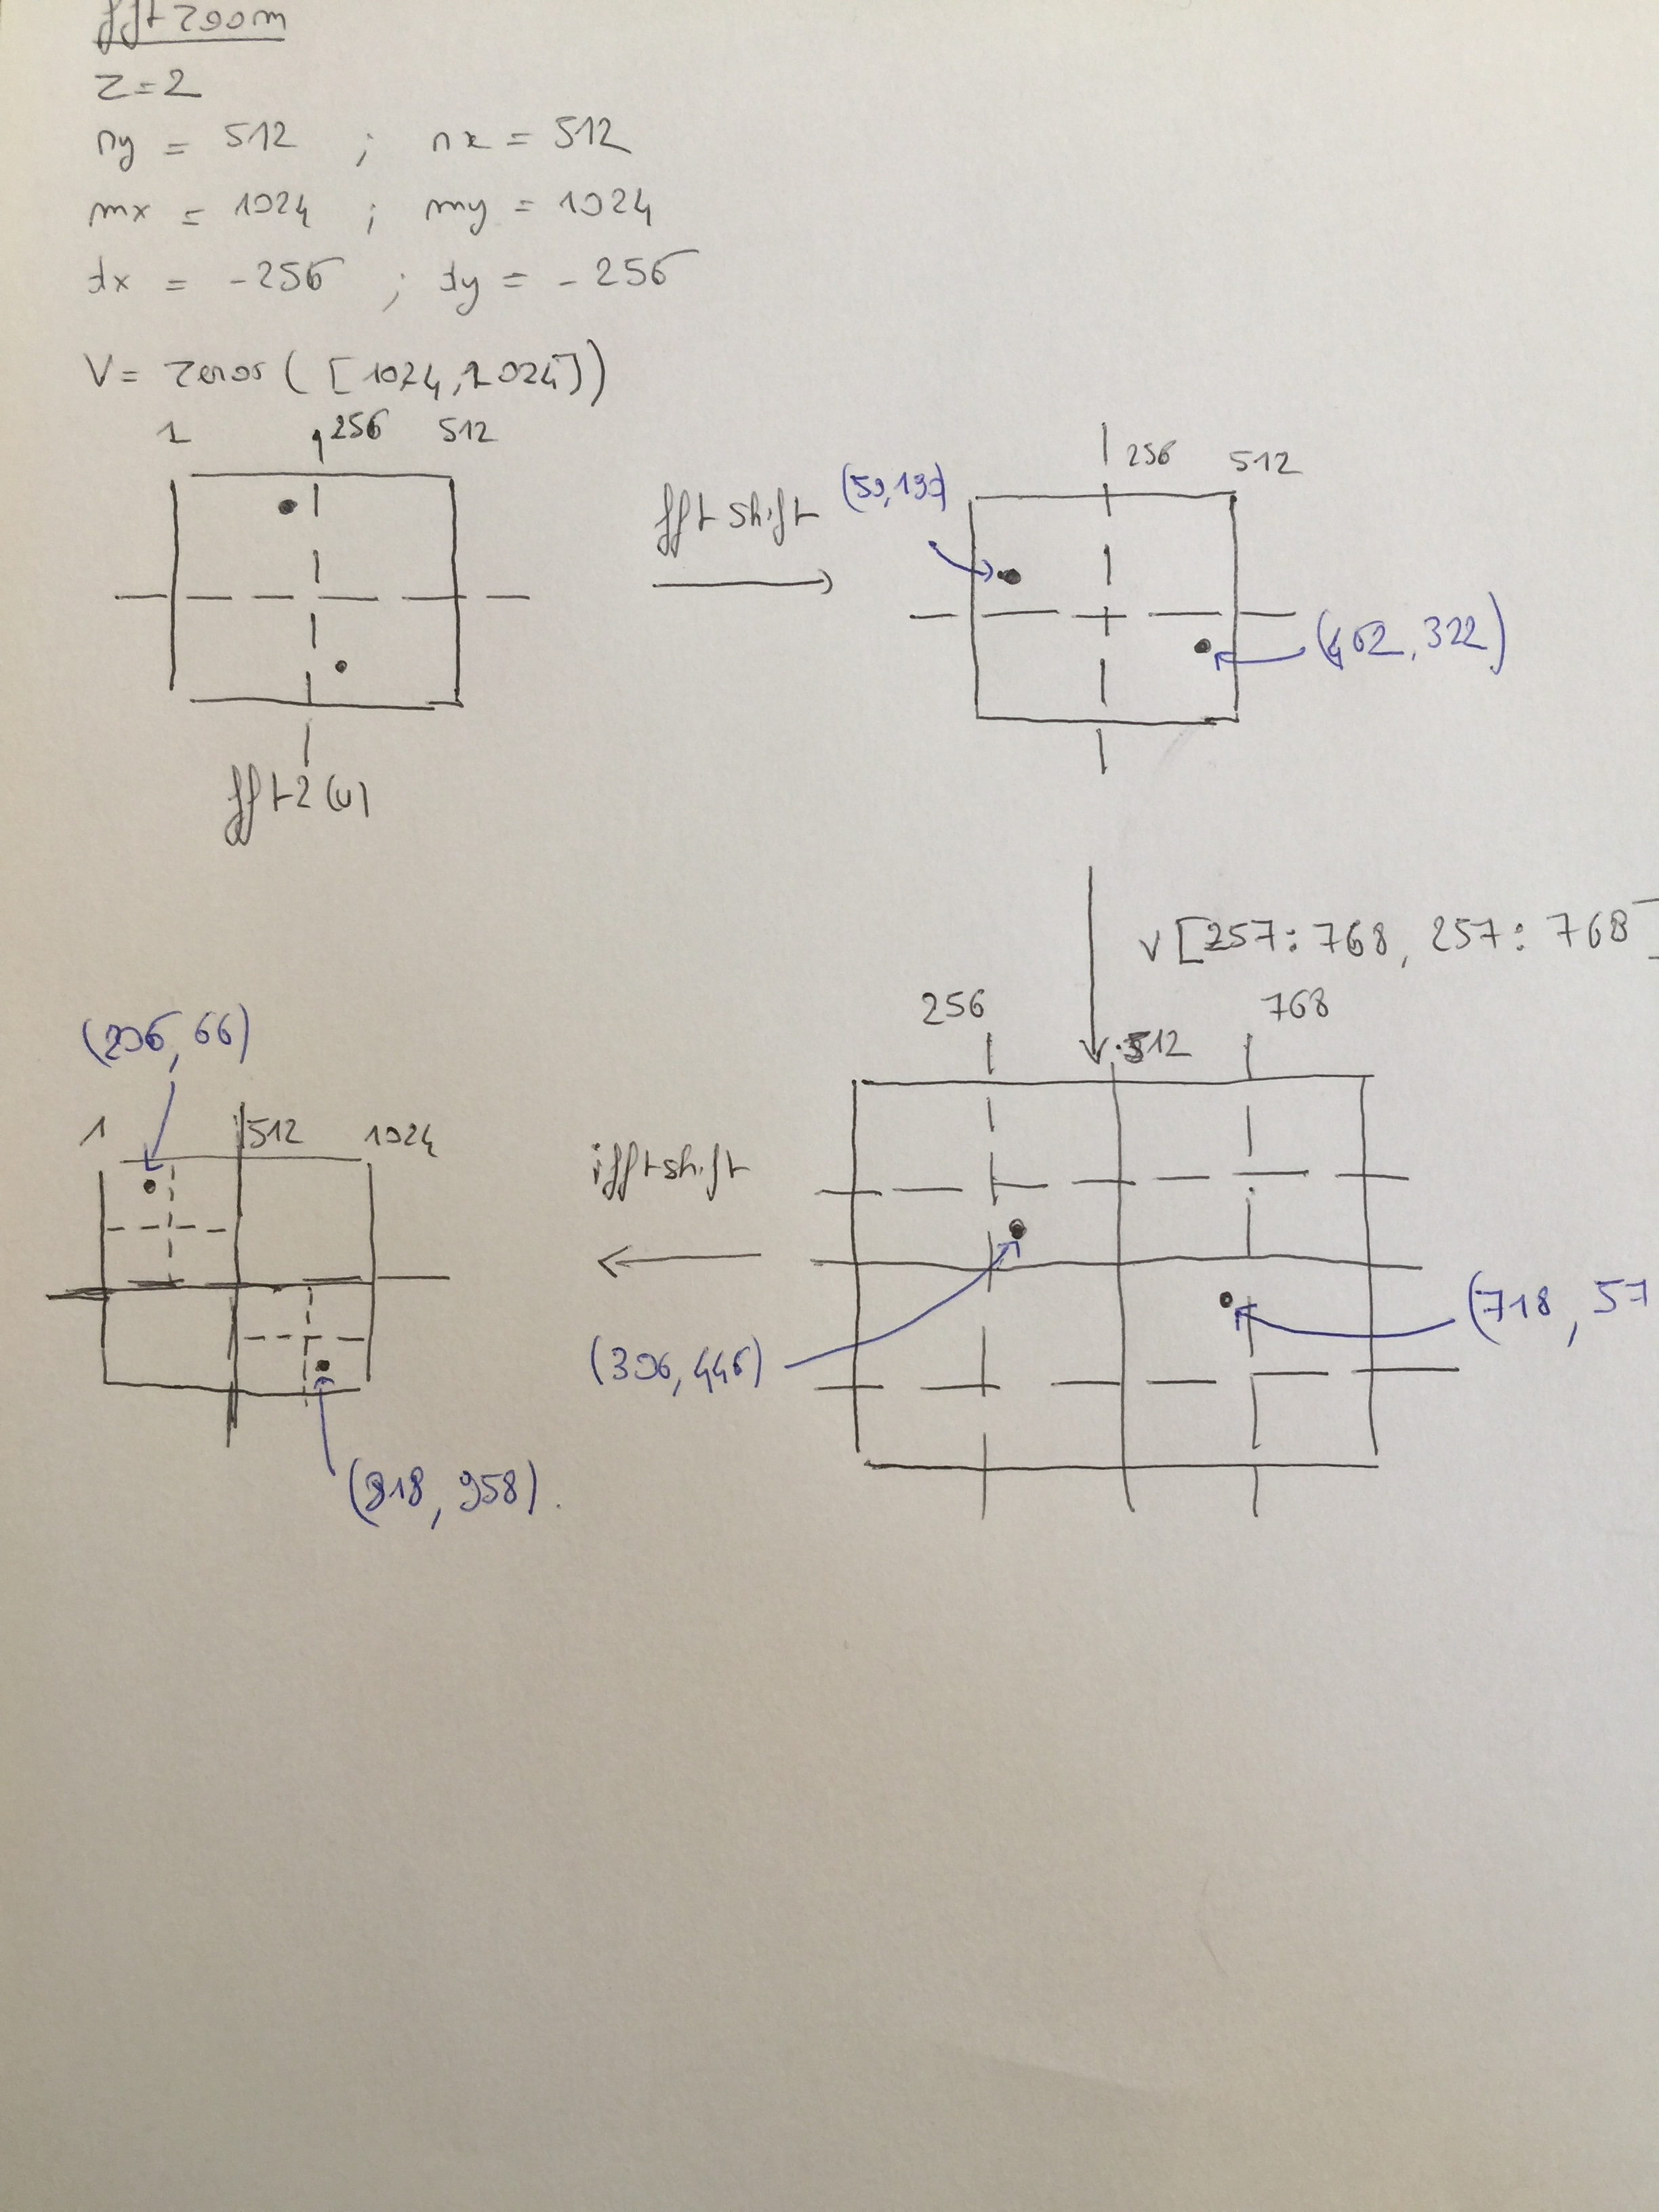
\includegraphics[width=10cm]{fft_zoom_scheme.png}
\caption{Schéma explicatif fftzoom}
\end{figure}

\pagebreak

Etant donné le schéma, l'expression de la matrice renvoyée par fftzoom(onde,2) est:
\begin{equation}
\forall p, q \in 1,\dots,1024 \qquad \text{fftzoom(onde,2)}[p,q] = \Re{\Big(\text{cte} \times 
e^{\frac{2i\pi66(p-1)}{1024}} e^{\frac{2i\pi206(q-1)}{1024}}\Big)}
\end{equation}

On peut donc recréer directement l'image 2 fois plus résolue par le code suivant:

\begin{lstlisting}[frame=single]
g = zeros(1024, 1024);
g(66, 206) = 2;
onde_fftzoom = real(ifft2(g));
imshow(onde_fftzoom, []);
\end{lstlisting}

\begin{figure}[!h]
\centering
\includegraphics[width=6cm]{ex_5_onde_zoom_recreate.png}
\caption{Image recréée}
\end{figure}

3) On définit la fonction souhaitée. 

\begin{lstlisting}[frame=single]
function v = gradn (u)
   [M,N] = size(u);
   v = zeros(M-1, N-1);
   for k=1:(M-1)
        for l=1:(N-1)
            v(k,l) = sqrt((u(k+1,l)-u(k,l))^2+(u(k, l+1)-u(k,l))^2);
        end
    end
endfunction
\end{lstlisting}

On l'applique à l'image nimes.pgm et on observe:

\begin{lstlisting}[frame=single]
u = double(imread("nimes.pgm"))/255;
imshow(u);
imshow(gradn(u));
\end{lstlisting}

\begin{figure}[!h]
\centering
\subfloat[Image nimes]{{\includegraphics[width=6cm]{ex_5_nimes.png}}}%
\qquad
\subfloat[Image norme gradient nimes]{{\includegraphics[width=6cm]{ex_5_gradn.png}}}%
\end{figure}

\end{document}

